\documentclass[tikz,border=12pt]{standalone}
\usepackage{amsmath,amssymb,amsfonts}
\usepackage{booktabs}
\usepackage{array}
\usepackage{colortbl}
\usepackage{xcolor}
\usetikzlibrary{arrows.meta,positioning,calc,fit,backgrounds,shapes.geometric}

% --- LaTikZ Standard Barrier-Free Palette ---
\definecolor{sciBlue}{HTML}{0072B2}
\definecolor{sciOrange}{HTML}{D55E00}
\definecolor{sciGreen}{HTML}{009E73}
\definecolor{sciPurple}{HTML}{CC79A7}
\definecolor{sciYellow}{HTML}{E69F00}
\definecolor{sciSky}{HTML}{56B4E9}
\definecolor{sciTeal}{HTML}{008B8B}
\definecolor{sciRed}{HTML}{C0392B}
\definecolor{sciDark}{HTML}{222222}
\definecolor{sciGray}{HTML}{7F8C8D}
\definecolor{sciLight}{HTML}{F8F9FA}
\definecolor{cardBg}{HTML}{FFFFFF}
\definecolor{cardBorder}{HTML}{D0D7DE}
\definecolor{hdrBg}{HTML}{0F2537}
\definecolor{rowAlt}{HTML}{F4F8FA}
\definecolor{goldStar}{HTML}{D4AF37}

\newcommand{\badge}[3]{%
  \tikz[baseline=-0.6ex]{%
    \node[rectangle, rounded corners=3pt, fill=#1!15, draw=#1!80, line width=0.5pt, inner sep=2pt, font=\scriptsize\sffamily\bfseries, text=#2] {#3};%
  }%
}

\begin{document}
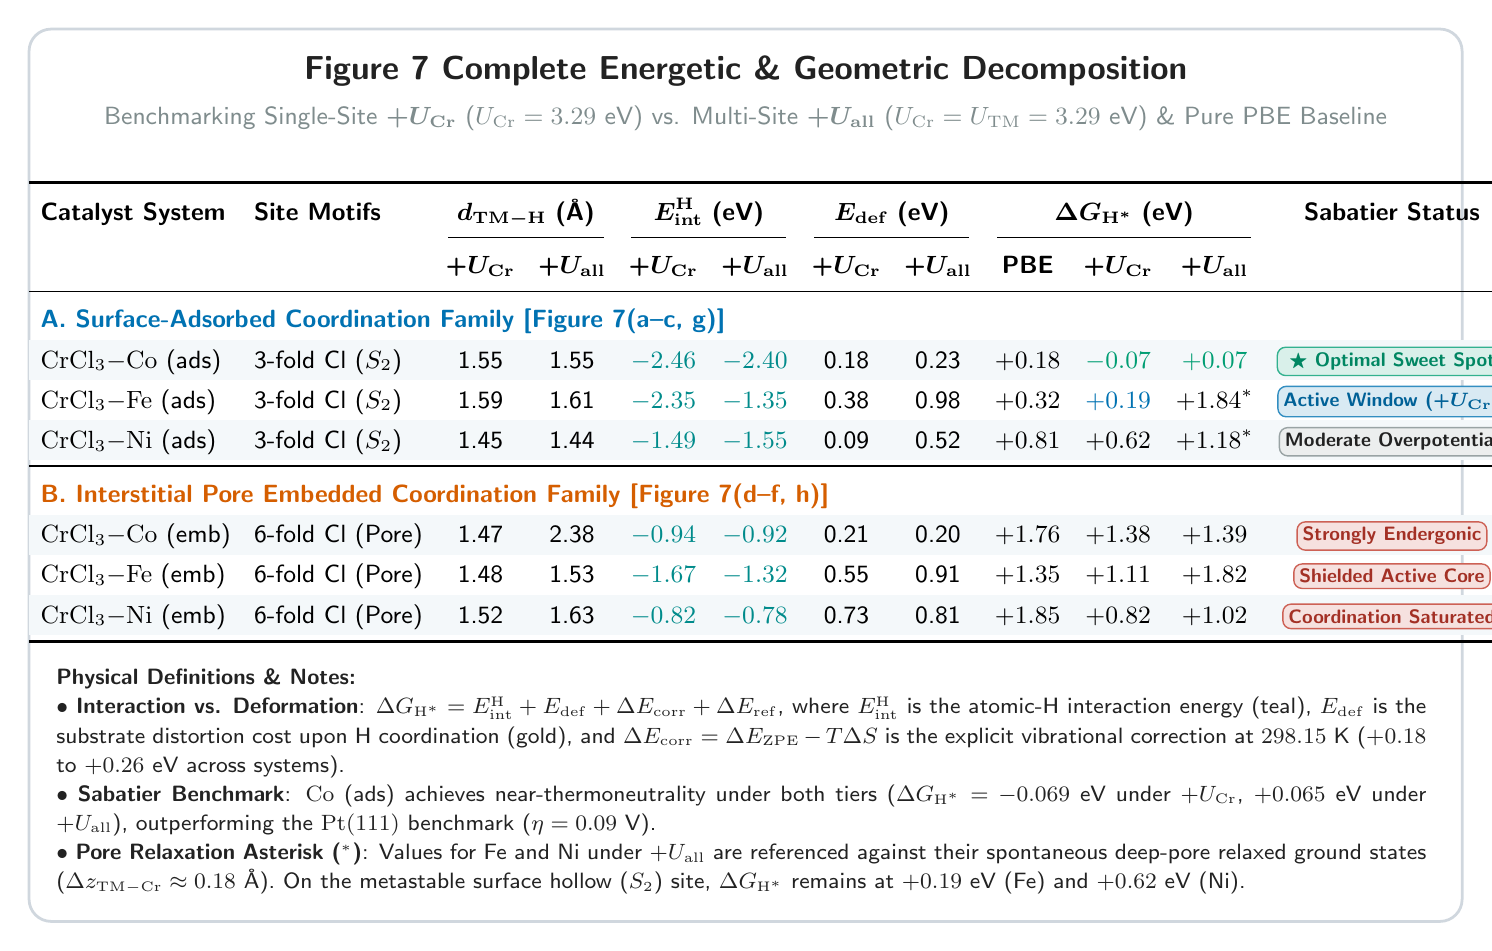
\begin{tikzpicture}[font=\sffamily, >=Stealth]

  % Main Card Outline
  \node[rectangle, draw=cardBorder, fill=cardBg, line width=1.0pt, rounded corners=8pt, inner sep=0pt] (maincard) {
    \begin{minipage}{18.2cm}
      \vspace{0.35cm}
      % -------------------------------------------------------------
      % Title Banner
      % -------------------------------------------------------------
      \begin{center}
        {\fontsize{13pt}{16pt}\selectfont \textbf{\color{sciDark} Figure 7 Complete Energetic \& Geometric Decomposition}}\\[0.15cm]
        {\fontsize{9pt}{12pt}\selectfont \color{sciGray} Benchmarking Single-Site $\boldsymbol{+U_{\mathrm{Cr}}}$ ($U_{\mathrm{Cr}}=3.29$~eV) vs. Multi-Site $\boldsymbol{+U_{\mathrm{all}}}$ ($U_{\mathrm{Cr}}=U_{\mathrm{TM}}=3.29$~eV) \& Pure PBE Baseline}
      \end{center}
      \vspace{0.25cm}

      % -------------------------------------------------------------
      % Table Body with Precise Cell Formatting
      % -------------------------------------------------------------
      \centering
      \small
      \setlength{\tabcolsep}{4.2pt}
      \renewcommand{\arraystretch}{1.32}
      \begin{tabular}{ll ccc ccc ccc c}
        \toprule[1.2pt]
        \textbf{Catalyst System} & \textbf{Site Motifs} & \multicolumn{2}{c}{$\boldsymbol{d_{\mathrm{TM-H}}}$ \textbf{(\AA)}} & \multicolumn{2}{c}{$\boldsymbol{E_{\mathrm{int}}^{\mathrm{H}}}$ \textbf{(eV)}} & \multicolumn{2}{c}{$\boldsymbol{E_{\mathrm{def}}}$ \textbf{(eV)}} & \multicolumn{3}{c}{$\boldsymbol{\Delta G_{\mathrm{H}^*}}$ \textbf{(eV)}} & \textbf{Sabatier Status} \\
        \cmidrule(lr){3-4} \cmidrule(lr){5-6} \cmidrule(lr){7-8} \cmidrule(lr){9-11}
        & & \textbf{+$\boldsymbol{U_{\mathrm{Cr}}}$} & \textbf{+$\boldsymbol{U_{\mathrm{all}}}$} & \textbf{+$\boldsymbol{U_{\mathrm{Cr}}}$} & \textbf{+$\boldsymbol{U_{\mathrm{all}}}$} & \textbf{+$\boldsymbol{U_{\mathrm{Cr}}}$} & \textbf{+$\boldsymbol{U_{\mathrm{all}}}$} & \textbf{PBE} & \textbf{+$\boldsymbol{U_{\mathrm{Cr}}}$} & \textbf{+$\boldsymbol{U_{\mathrm{all}}}$} & \\
        \midrule
        \multicolumn{12}{l}{\textbf{\color{sciBlue} A. Surface-Adsorbed Coordination Family [Figure 7(a--c, g)]}} \\
        \rowcolor{rowAlt}
        $\mathrm{CrCl}_3\mathrm{-Co}$ (ads) & 3-fold Cl ($S_2$) & 1.55 & 1.55 & \color{sciTeal}$-2.46$ & \color{sciTeal}$-2.40$ & 0.18 & 0.23 & $+0.18$ & \textbf{\color{sciGreen}$-0.07$} & \textbf{\color{sciGreen}$+0.07$} & \badge{sciGreen}{sciGreen!85!black}{\;$\bigstar$ Optimal Sweet Spot\;} \\
        $\mathrm{CrCl}_3\mathrm{-Fe}$ (ads) & 3-fold Cl ($S_2$) & 1.59 & 1.61 & \color{sciTeal}$-2.35$ & \color{sciTeal}$-1.35$ & 0.38 & 0.98 & $+0.32$ & \textbf{\color{sciBlue}$+0.19$} & $+1.84^*$ & \badge{sciBlue}{sciBlue!85!black}{Active Window (+$\boldsymbol{U_{\mathrm{Cr}}}$)} \\
        \rowcolor{rowAlt}
        $\mathrm{CrCl}_3\mathrm{-Ni}$ (ads) & 3-fold Cl ($S_2$) & 1.45 & 1.44 & \color{sciTeal}$-1.49$ & \color{sciTeal}$-1.55$ & 0.09 & 0.52 & $+0.81$ & $+0.62$ & $+1.18^*$ & \badge{sciGray}{sciDark}{Moderate Overpotential} \\
        \midrule
        \multicolumn{12}{l}{\textbf{\color{sciOrange} B. Interstitial Pore Embedded Coordination Family [Figure 7(d--f, h)]}} \\
        \rowcolor{rowAlt}
        $\mathrm{CrCl}_3\mathrm{-Co}$ (emb) & 6-fold Cl (Pore) & 1.47 & 2.38 & \color{sciTeal}$-0.94$ & \color{sciTeal}$-0.92$ & 0.21 & 0.20 & $+1.76$ & $+1.38$ & $+1.39$ & \badge{sciRed}{sciRed!85!black}{Strongly Endergonic} \\
        $\mathrm{CrCl}_3\mathrm{-Fe}$ (emb) & 6-fold Cl (Pore) & 1.48 & 1.53 & \color{sciTeal}$-1.67$ & \color{sciTeal}$-1.32$ & 0.55 & 0.91 & $+1.35$ & $+1.11$ & $+1.82$ & \badge{sciRed}{sciRed!85!black}{Shielded Active Core} \\
        \rowcolor{rowAlt}
        $\mathrm{CrCl}_3\mathrm{-Ni}$ (emb) & 6-fold Cl (Pore) & 1.52 & 1.63 & \color{sciTeal}$-0.82$ & \color{sciTeal}$-0.78$ & 0.73 & 0.81 & $+1.85$ & $+0.82$ & $+1.02$ & \badge{sciRed}{sciRed!85!black}{Coordination Saturated} \\
        \bottomrule[1.2pt]
      \end{tabular}

      \vspace{0.3cm}
      % -------------------------------------------------------------
      % Explanatory Footer Cards
      % -------------------------------------------------------------
      \begin{minipage}{17.4cm}
        \fontsize{7.8pt}{10.5pt}\selectfont \color{sciDark}
        \textbf{Physical Definitions \& Notes:}\\
        $\bullet$ \textbf{Interaction vs. Deformation}: $\Delta G_{\mathrm{H}^*} = E_{\mathrm{int}}^{\mathrm{H}} + E_{\mathrm{def}} + \Delta E_{\mathrm{corr}} + \Delta E_{\mathrm{ref}}$, where $E_{\mathrm{int}}^{\mathrm{H}}$ is the atomic-H interaction energy (teal), $E_{\mathrm{def}}$ is the substrate distortion cost upon H coordination (gold), and $\Delta E_{\mathrm{corr}} = \Delta E_{\mathrm{ZPE}} - T\Delta S$ is the explicit vibrational correction at $298.15$~K ($+0.18$ to $+0.26$~eV across systems).\\
        $\bullet$ \textbf{Sabatier Benchmark}: $\mathrm{Co}$ (ads) achieves near-thermoneutrality under both tiers ($\Delta G_{\mathrm{H}^*} = -0.069$~eV under $+U_{\mathrm{Cr}}$, $+0.065$~eV under $+U_{\mathrm{all}}$), outperforming the $\mathrm{Pt}(111)$ benchmark ($\eta = 0.09$~V).\\
        $\bullet$ \textbf{Pore Relaxation Asterisk ($^*$)}: Values for Fe and Ni under $+U_{\mathrm{all}}$ are referenced against their spontaneous deep-pore relaxed ground states ($\Delta z_{\mathrm{TM-Cr}} \approx 0.18$~\AA). On the metastable surface hollow ($S_2$) site, $\Delta G_{\mathrm{H}^*}$ remains at $+0.19$~eV (Fe) and $+0.62$~eV (Ni).
      \end{minipage}
      \vspace{0.35cm}
    \end{minipage}
  };

\end{tikzpicture}
\end{document}
